\documentclass[11pt,letterpaper,titlepage]{article}

%================== Document nomenclature
\newcommand{\DOCSUBJT}{Whitepaper: }   %Put document subject here
\newcommand{\DOCTITLE}{                      %Put document title here
	Diffusion Solver in ChiTech
}       
\newcommand{\DOCDATE} {August, 2018}         %Put document date here
\newcommand{\DOCREV}  {Rev 1.00}             %Put revision number here

%================== Misc Settings
\usepackage{fancyhdr}
\usepackage[left=0.75in, right=0.75in, bottom=1.0in]{geometry}
\usepackage{lastpage}
\usepackage{titleref}
\usepackage{booktabs}
\usepackage{appendix}
\usepackage{ stmaryrd }

\appendixtitleon
\appendixtitletocon

\makeatletter

%================== List of figures and tables mods
\usepackage{tocloft}
\usepackage[labelfont=bf]{caption}

\renewcommand{\cftfigpresnum}{Figure\ }
\renewcommand{\cfttabpresnum}{Table\ }

\newlength{\mylenf}
\settowidth{\mylenf}{\cftfigpresnum}
\setlength{\cftfignumwidth}{\dimexpr\mylenf+1.5em}
\setlength{\cfttabnumwidth}{\dimexpr\mylenf+1.5em}



%=================== Graphics
\usepackage{graphicx}
\usepackage[breakwords]{truncate}
\usepackage{float}
\usepackage{array}
\usepackage{amsmath}
\usepackage{mdframed}
\usepackage{fancyvrb}
\usepackage{float}
\usepackage{cancel}
\usepackage{amssymb}
\graphicspath{ {images/} }
\usepackage[usenames,dvipsnames,svgnames,table]{xcolor}
\usepackage[defaultlines=2,all]{nowidow}
\usepackage{listings}
\usepackage{color}
\definecolor{Brown}{cmyk}{0,0.81,1,0.60}
\definecolor{OliveGreen}{cmyk}{0.64,0,0.95,0.40}
\definecolor{CadetBlue}{cmyk}{0.62,0.57,0.23,0}
\usepackage{pdflscape}
\usepackage{relsize}
\usepackage{verbatim}
\usepackage{tabto}
\usepackage{upgreek}
\usepackage{enumitem}

\usepackage{mathtools}

%=================== Settings
\renewcommand{\baselinestretch}{1.2}
\definecolor{gray}{rgb}{0.4 0.4 0.4}
\newcommand{\stimes}{{\times}}

\newcommand*{\ldblbrace}{\{\mskip-5mu\{}
\newcommand*{\rdblbrace}{\}\mskip-5mu\}}


\newcommand{\xmltag}[1]{\textcolor{blue}{ \texttt{#1}} }
\newcommand{\xmloption}[1]{\textcolor{ao(english)}{ \texttt{#1}} }

%================== Code syntax highlighting
\lstset{language=C++,frame=ltrb,framesep=2pt,basicstyle=\linespread{0.8} \small,
	keywordstyle=\ttfamily\color{OliveGreen},
	identifierstyle=\ttfamily\color{CadetBlue}\bfseries,
	commentstyle=\color{Brown},
	stringstyle=\ttfamily,
	showstringspaces=true,
	tabsize=2,}

\newcommand{\bOmega}{\mathcal{D}}

\setlength\parindent{0pt}

%================== Section numbers with equation numbers
\numberwithin{equation}{section}

\begin{document}

\begin{titlepage}
	\pagestyle{fancy}
	\vspace*{1.0cm}
	\centering
	\vspace{1cm}
	\vspace{.25cm}
	{\Large\bfseries  \DOCSUBJT \par} 
	{\Large\bfseries \DOCTITLE  \par}
	\vspace{1cm}
	{\Large \DOCDATE \par}
	\vspace{1.0cm}
	{\Large Jan Vermaak \par}
	{\Large \DOCREV \par}
	\begin{center}
		\begin{minipage}[c]{0.45\textwidth}
			\begin{figure}[H]
				
				
\includegraphics[width=3in]{Logo2_Medium.png}
			\end{figure}
		\end{minipage}
	\end{center}

\end{titlepage}	


\pagestyle{fancy}
\rfoot{Page \thepage \ of \pageref{LastPage}}
\cfoot{}
\lfoot{\truncate{14cm}{\DOCTITLE}}
\rhead{}
\chead{\currentname}
\lhead{}
\renewcommand{\footrulewidth}{0.4pt}

\begin{comment}
\tableofcontents
\addtocontents{toc}{~\hfill\textbf{Page}\par}

\listoffigures
\listoftables

\end{comment}
\chead{Weak form}	

%#########################################################################
\newpage
\section{The Weak form of the general Diffusion Equation}
The diffusion solver handles the solution of the diffusion equation of the form

\begin{equation} \label{eq:diffeq}
-\nabla (D\nabla\phi) + \sigma_a \phi = q
\end{equation}
\newline
\noindent
over the domain $\mathcal{D}$ and with any set of boundary conditions on the boundary $\partial \mathcal{D}$. This form is suitable for physical processes like heat transfer when $\sigma_a = 0$ and processes like neutron diffusion when $\sigma_a \ne 0$.
\newline \newline
We now proceed with multiplying with $\varphi_i$, a function mapping eq. \ref{eq:diffeq} to a trial space $\mathcal{D}_i$ for which we require that

\begin{equation} \label{eq:trial}
\int_{\bOmega_i} \biggr( 
-\varphi_i\nabla (D\nabla\phi) 
\biggr).dV 
+ \int_{\bOmega_i} ( 
\varphi_i\sigma_a  \phi 
  ).dV
= \int_{\bOmega_i} (\varphi_i q).dV.
\end{equation}
\newline
In this equation we note that, from the product rule we have

\begin{align*}
\frac{d(fg)}{dx} &= \frac{df}{dx}\cdot g + f\cdot \frac{dg}{dx} \\
\therefore 
\int \frac{d(fg)}{dx} .dx&= \int \frac{df}{dx}\cdot g.dx + 
\int f\cdot \frac{dg}{dx}.dx
\end{align*}
\newline
Applying this as an analogy with $f=\varphi$ and $g=D\nabla \phi$ we get

\begin{equation}\label{eq:IntegrateByParts}
\begin{aligned}
\int_{\bOmega_i} \nabla( \varphi_i D\nabla \phi) .dV&=
\int_{\bOmega_i} \nabla \varphi_i\cdot D\nabla \phi.dV + 
\int_{\bOmega_i} \varphi_i\cdot \nabla(D\nabla \phi).dV \\
\therefore
-\int_{\bOmega_i} \biggr(
\varphi_i\cdot \nabla(D\nabla \phi).dV
\biggr) &=
\int_{\bOmega_i} \nabla \varphi_i\cdot D\nabla \phi.dV
-\int_{\bOmega_i} \nabla( \varphi_i D\nabla \phi) .dV
\end{aligned}
\end{equation}
\newline
Now applying Gauss's Divergence theorem on the last term we have
\begin{align}\label{eq:GaussDiv}
\int_{\bOmega_i} \nabla( \varphi_i D\nabla \phi) .dV &=
\int_{\partial \bOmega} \hat{n}\cdot \varphi_i D\nabla \phi . dA
\end{align}
\newline
which we can place in equation \ref{eq:IntegrateByParts} and then subsequently into equation \ref{eq:trial} which leads to the weak form

\begin{align}\label{eq:weakform}
\Aboxed{
\int_{\bOmega_i} \biggr(
\nabla \varphi_i\cdot D\nabla \phi
+
\varphi_i\sigma_a  \phi 
\biggr).dV 
- 
\int_{\partial \bOmega}\biggr( 
\hat{n}\cdot \varphi_i D\nabla \phi 
\biggr). dA
= \int_{\bOmega_i} (\varphi_i q).dV
}.
\end{align}

\newpage
\chead{Basis functions}
\section{Application of basis functions}
Consider $\phi$ approximated by the contributions of basis functions, $N_j$, and associated coefficients $\phi_j$, i.e.
\begin{align}
\phi \approx \phi_h = \sum_{j=0}^N \phi_j N_j.
\end{align}
Also consider the source $q$ as being a combination of: a constant-per-element component, $q_c$, and a non-constant-per-element component, $q_{nc}$. The non-constant component can then also be expandedusing basis functions and coefficients
\begin{align}
q_{nc} \approx q_{nc,h} = \sum_{j=0}^N q_{nc,j} N_j.
\end{align}
\newline
Equation \ref{eq:weakform} now becomes 

\begin{align*}
\begin{aligned}
&\int_{\bOmega_i} \biggr(
\nabla \varphi_i\cdot D\nabla (\sum_{j=0}^N \phi_j N_j)
+
\varphi_i\sigma_a  (\sum_{j=0}^N \phi_j N_j)
\biggr).dV
-
\int_{\partial \bOmega}\biggr( 
\mathbf{\hat{n}}\cdot \varphi_i D\nabla (\sum_{j=0}^N \phi_j N_j) 
\biggr). dA
\\
&= \int_{\bOmega_i} \varphi_i q_c.dV + \int_{\bOmega_i} \varphi_i (\sum_{j=0}^N q_{nc,j} N_j).dV 
\end{aligned}
\end{align*}
\noindent after which we can move the $\nabla$ operator such that
\begin{align*}
\begin{aligned}
&\int_{\bOmega_i} \biggr(
\nabla \varphi_i\cdot D (\sum_{j=0}^N \phi_j \nabla N_j)
+ 
\varphi_i\sigma_a  (\sum_{j=0}^N \phi_j N_j)
\biggr).dV
-
\int_{\partial \bOmega}\biggr( 
\mathbf{\hat{n}}\cdot \varphi_i D (\sum_{j=0}^N \phi_j \nabla N_j) 
\biggr). dA 
\\
&= \int_{\bOmega_i} \varphi_i q_c.dV+
 \int_{\bOmega_i} \varphi_i (\sum_{j=0}^N q_{nc,j} N_j).dV 
\end{aligned}
\end{align*}
\newline
We now take into account that each integral over a trial space $\bOmega_i$ is a summation over all the elements $\mathcal{K}$ that fall within this space. I.e.
\newline
\newline
\textbf{Trial space i}

\begin{equation*}
\begin{aligned}
&\sum^K \biggr[
\int_{\bOmega_i} \biggr(
\nabla \varphi_i\cdot D (\sum_{j=0}^N \phi_j \nabla N_j)
+
\varphi_i\sigma_a  (\sum_{j=0}^N \phi_j N_j)
\biggr).dV
-
\int_{\partial \bOmega}\biggr( 
\mathbf{\hat{n}}\cdot \varphi_i D (\sum_{j=0}^N \phi_j \nabla N_j) 
\biggr). dA \biggr]
\\
&=\sum^K \biggr[
 \int_{\bOmega_i} (\varphi_i q_c).dV
 +
  \int_{\bOmega_i} \varphi_i (\sum_{j=0}^N q_{nc,j} N_j).dV 
  \biggr]
\end{aligned}
\end{equation*}
Rearranging
\begin{equation*}
\begin{aligned}
&\sum^K
\sum_{j=0}^N
 \biggr[
\int_{\bOmega_i} \biggr(
\nabla \varphi_i\cdot D ( \phi_j \nabla N_j)
+
\varphi_i\sigma_a  ( \phi_j N_j)
\biggr).dV
-
\int_{\partial \bOmega}\biggr( 
\mathbf{\hat{n}}\cdot \varphi_i D ( \phi_j \nabla N_j) 
\biggr). dA \biggr]
\\
&=\sum^K 
\biggr[
 \int_{\bOmega_i} (\varphi_i q_c).dV
\biggr]
 +
 \sum^K
 \sum_{j=0}^N
 \biggr[
  \int_{\bOmega_i} \varphi_i ( q_{nc,j} N_j).dV 
  \biggr]
\end{aligned}
\end{equation*}

\begin{equation*}
\begin{aligned}
\therefore
&\sum^K
\sum_{j=0}^N \phi_j
 \biggr[ 
D \int_{\bOmega_i} 
\nabla \varphi_i \cdot  \nabla N_j.dV
+
\sigma_a \int_{\bOmega_i}  \varphi_i N_j
.dV
-
D \ \hat{n} \cdot \int_{\partial \bOmega}
 \varphi_i \nabla N_j
. dA \biggr]
\\
&=\sum^K 
\biggr[q_c
 \int_{\bOmega_i} \varphi_i .dV 
 \biggr]
 +
 \sum^K
 \sum_{j=0}^N 
 \biggr[q_{nc,j}
  \int_{\bOmega_i} \varphi_i  N_j.dV 
  \biggr]
\end{aligned}
\end{equation*}
\newline
By using the same shape functions for the test functions as was used for the basis functions, $\varphi_i = N_i$, we have the following, Galerkin-form of the equations
\begin{equation}
\begin{aligned}
\therefore
&\sum^K
\sum_{j=0}^N \phi_j
 \biggr[ 
D \int_{\bOmega_i} 
\nabla N_i \cdot  \nabla N_j.dV
+
\sigma_a \int_{\bOmega_i}  N_i N_j
.dV
-
D \ \hat{n} \cdot \int_{\partial \bOmega}
 N_i \nabla N_j
. dA \biggr]
\\
&=\sum^K 
\biggr[q_c
 \int_{\bOmega_i} N_i .dV 
 \biggr]
 +
 \sum^K
 \sum_{j=0}^N 
 \biggr[q_{nc,j}
  \int_{\bOmega_i} N_i  N_j.dV 
  \biggr]
\end{aligned}
\end{equation}
\newline
Computing the integrals of different combinations of the shape functions is specific to the type of element used, i.e. 1D slab, 2D triangle, 2D polygon, 3D tetrahedron, 3D polyhedron, etc. This information is contained in relevant whitepapers.

\newpage
\chead{CFEM}
\section{Continuous Finite Element Method (CFEM)}

The use of continuous basis functions, as well as the test functions being the same as the basis functions gives rise to the notion of a Galerkin method denoted as the Continous Finite Element Method (CFEM).

\subsection{Assembling the linear system of equations}
With each trial space representing an equation, we can assemble a row of a matrix $A$ and an associated entry in the vector $\mathbf{b}$ as
 
\vspace{0.25cm}
\textbf{For each element k, for each DOF-$i$, for each DOF-$j$}
\begin{equation}
\begin{aligned}
a_{ij} &=a_{ij} +  D \int_{\bOmega_i} \nabla N_i  \cdot  \nabla N_j .dV + 
\sigma_a \int_{\bOmega_i} N_i N_j.dV -
D \  \hat{n} \cdot \int_{\partial \bOmega} N_i  \nabla N_j .dA 
\end{aligned}
\end{equation}
\begin{equation}
\begin{aligned}
b_i &= b_i 
+ q_{nc,j} \int_{\bOmega_i}  N_i  N_j .dV
\end{aligned}
\end{equation}

\textbf{For each element k, for each DOF-$i$}
\begin{equation}
\begin{aligned}
b_i &= b_i + q_c \int_{\bOmega_i} N_i   .dV 
\end{aligned}
\end{equation}

\subsection{Boundary conditions}
There are 2 primary types of boundary conditions implemented in ChiTech; \textbf{Dirichlet} type boundary conditions and \textbf{Robin} type boundary conditions.

\subsubsection{Robin and Neumann type boundary conditions}
A \textbf{Neumann} boundary condition takes the form

\begin{equation*}
-D \hat{n} \cdot \nabla \phi = f \quad \quad \text{on } \partial \bOmega
\end{equation*}

where $f$ represents a function. This representation is trivial to implement in the equation for $a_{ij}$ since it essentially means the integral on the boundary is a known and can hence be moved to the right hand side. Hence the equations to do so simply become

\begin{equation*}
\begin{aligned}
a_{ij} &=a_{ij} +  D \int_{\bOmega_i} \nabla N_i  \cdot  \nabla N_j .dV + 
\sigma_a \int_{\bOmega_i} N_i N_j.dV - \cancel{
D \  \hat{n} \cdot \int_{\partial \bOmega} N_i  \nabla N_j .dA} \\
b_i &= b_i 
+ q_{nc,j} \int_{\bOmega_i}  N_i  N_j .dV - f_j \int_{\partial\bOmega}  N_i  N_j .dA
\end{aligned}
\end{equation*}
and the rest remaining untouched.
\newline
\newline
In the case of a \textbf{Robin} boundary condition the form is similar;

\begin{equation*}
\alpha \phi+\beta D \hat{n} \cdot \nabla \phi = f \quad \quad \text{on } \partial \bOmega
\end{equation*}

however, this time around there is a component still dependent on $\phi$ which must remain on the left hand side. The equations are

\begin{equation*}
\begin{aligned}
a_{ij} &=a_{ij} +  D \int_{\bOmega_i} \nabla N_i  \cdot  \nabla N_j .dV + 
\sigma_a \int_{\bOmega_i} N_i N_j.dV - \cancel{
D \  \hat{n} \cdot \int_{\partial \bOmega} N_i  \nabla N_j .dA} 
+ 
\frac{\alpha}{\beta} \int_{\partial\bOmega} N_i N_j.dA\\
b_i &= b_i 
+ q_{nc,j} \int_{\bOmega_i}  N_i  N_j .dV + \frac{f_j}{\beta} \int_{\partial\bOmega}  N_i  b_j .dV
\end{aligned}
\end{equation*}
\newline
With this notation we can see that by using a Robin boundary condition with $\alpha=0$ and $\beta=-1$ we can essentially specify a Neumann boundary condition.
\newline
\newline
The versatility of this boundary condition can also be extended to \textbf{Vacuum} boundary conditions in neutron diffusion which take the form

\begin{equation*}
\frac{1}{4}\phi + \frac{1}{2}D\hat{n}\cdot\nabla\phi = 0 \quad \quad \text{on } \partial \bOmega
\end{equation*}

representing a zero incoming current. It is simple to see that using the values $\alpha = \frac{1}{4}$, $\beta=\frac{1}{2}$ and $f=0$ one can specify a vacuum boundary condition using a Robin boundary condition.

\subsubsection{Dirichlet type boundary conditions}
The Robin type boundary conditions does not have the potential to destroy the symmetry of the matrix. \textbf{Dirichlet} boundary conditions on the other hand do have this potential. The Dirichlet boundary conditions takes the simple form

\begin{equation*}
\phi = c \quad \quad \text{on } \partial \bOmega.
\end{equation*}

Since none of the weak form equations have components of this form there is only one possible contribution to $a_{ij}$ and that is

\begin{equation*}
\begin{aligned}
&a_{ii} \mathbf{=} 1 \quad \quad a_{ij}=0\\
&b_i = c
\end{aligned}
\end{equation*}

Now, it is fairly trivial in theory to apply this process, however, with the finite element method normally assembling the matrix element-by-element the dirichlet boundary conditions will have to be applied after the element-by-element assembly. Additionally, the dirichlet process zeros out the non-diagonal columns of the given row. This is a problem because the rest of the element-by-element assembly connected other DOFs to the dirichlet DOF via the columns of their respective rows and hence if we do but zero out the non-diagonal components of the matrix row then we are left with a \textbf{non-symmetric} matrix.
\newline
\newline
In ChiTech the whole mess of Dirichlet boundary conditions is handled by modifying the element-by-element assembly process to never connect DOFs to the known dirichlet nodes. For a better understanding of how this is done please consult the coding implementation section.

\vspace{0.5cm}
\subsection{Coding implementation}
Currently 3 different geometries are implemented in ChiTech. For each geometry a subtle difference needs to be implemented, however, the code sequence is essentially identical. As a reference we will use only a 2D polygon but the overall code implementation is the same for all geometries. Let us now consider a simple 2D arrangement of $4{\times}4$ cells as shown in Figure \ref{fig:fourbyfour} below. The solution is defined on the nodes of the mesh and cells are distributed on processors depicted with colors.

\begin{figure}[H]
\centering
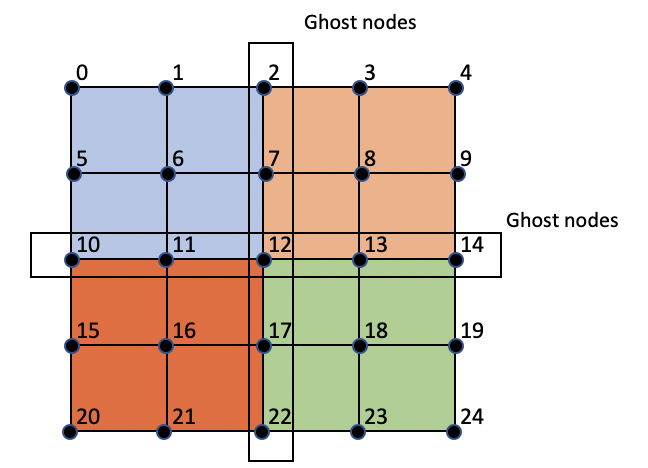
\includegraphics[width=0.5\linewidth]{Figures/FourByFour}
\caption{Simple CFEM arrangement of cells colored by processor ownership.}
\label{fig:fourbyfour}
\end{figure}

\subsubsection{Nodal Reordering}

This cell and processor arrangement results in a very disjointed matrix representation which is problematic for most parallel implementations and also results in the matrix having a very large bandwidth. To remedy this a \textbf{CFEM nodal re-ordering} is applied to the nodes of the mesh (\xmltag{ReorderNodesPWLC}). This process is a two stage process:
\newline
\newline
\textbf{Stage 1:}
\begin{itemize}
\item First all the nodes relevant to a process is collected into a set of exclusive and non-exclusive nodes. This involves a loop over all the degrees of freedom associated with a local cell.
\item Another loop is executed over local cells, however, this time we loop over faces and face DOFs. If a face is on a process boundary then node indices associated with all the face DOFs are removed from the exclusive non-exclusive node set and placed in a ghost-node set.
\item A ring communication is then used to communicate all the ghost nodes from location $i$ to location $i+1$ with the last location ending up with the complete list of ghost nodes. 
\item The last location then broadcasts the completed ghost node set to all other locations.
\end{itemize}

\textbf{Stage 2:}
\begin{itemize}
\item The ghost nodes is broken into $2P-2$ pieces (2 pieces per location, first and last location gets only 1 piece). If the amount of ghost nodes are not divisible they are stored as the remainder which will get subdivided between the first and last location.
\item With this information in hand each processor can determine the portion of the matrix it owns provided it knows the starting row. At this point only the first processor knows its ownership start ... its row 0. Therefore we initiate another ring communication. Each location takes its starting location, adds the local exclusive nodes, then the portion of the ghost nodes its been given and then send the next location its starting location.
\item Perform the mapping of original node indexes to distributed node indices.
\end{itemize}

This process can be visualized as depicted in Figure \ref{fig:CFEMReordering} below. The ordering allows for minimal communication between processes and overall low bandwidth when the amount of rows per processor is small. If further bandwidth reduction is required then a suitable reordering is required per process to reorder the exclusive nodes.

\begin{figure}[H]
\centering
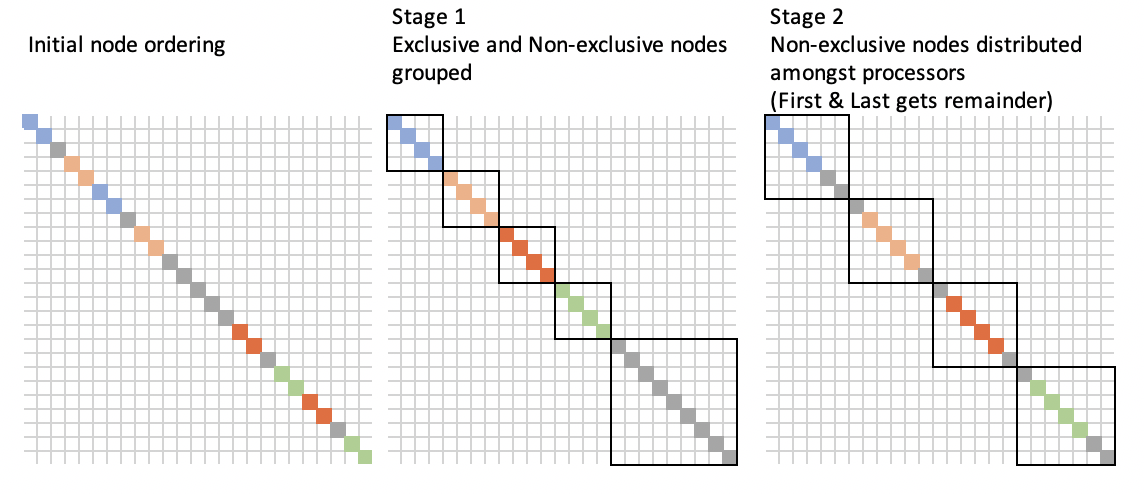
\includegraphics[width=0.9\linewidth]{Figures/CFEMReordering}
\caption{Stages of node ordering for CFEM.}
\label{fig:CFEMReordering}
\end{figure}

\subsubsection{Catching nodes on Dirichlet boundaries}
As was discussed in the previous section, the matrix assembly needs to be modified when nodes are on a Dirichlet boundary. Therefore we preprocess the faces to find nodes that are on such boundaries. Note that we loop over faces and only flag nodes if they are on a boundary.
\newline
\newline
\textbf{Defined in }\xmltag{diffusion\_solver\_01c\_init\_pwlc.cc}
\begin{lstlisting}[language=c++]
//================================== Check if i is on boundary
for (int i=0; i<poly_cell->v_indices.size(); i++)
{
	for (int e=0; e<poly_cell->edges.size(); e++)
	{
	  if (poly_cell->edges[e][2]<0)
	  {
	    int v0_index =
	      mesher->MapNode(poly_cell->edges[e][0]);
	    int v1_index =
	      mesher->MapNode(poly_cell->edges[e][1]);
	    if ((ir == v0_index) || (ir == v1_index))
	    {
	      int boundary_type =
	        boundaries[abs(poly_cell->edges[e][2])-1]->type;
	      if (boundary_type == DIFFUSION_DIRICHLET)
	      {
	        nodal_boundary_numbers[ir]=poly_cell->edges[e][2];
	      }
	      break;
	    } //if ir part of face
	  }
	}
}//for vertices i
\end{lstlisting}

\subsubsection{Estimating the sparsity pattern}
In order to improve memory allocation efficiency it is important to have a good estimation of the sparsity pattern of the matrix, specifically the number of non-zeros per row. The estimation is perfect if we can exactly estimate the amount of non-zeros per row, not perfect but good if we over-estimate it and poor if we under-estimate it.
\newline
\newline
\textbf{Defined in }\xmltag{diffusion\_solver\_01c\_init\_pwlc.cc}
\begin{lstlisting}[language=c++]
//======================================= Set nodal connections
for (int i=0; i<poly_cell->v_indices.size(); i++)
{
	std::vector<int>* node_links = nodal_connections[ir];
	for (int j=0; j<poly_cell->v_indices.size(); j++)
	{
	  int jr = mesher->MapNode(poly_cell->v_indices[j]);
	
	  //====================== Check for duplicates
	  bool already_there = false;
	  for (int k=0; k<node_links->size(); k++)
	  {
	    if ((*node_links)[k] == jr)
	    {already_there = true; break;}
	  }
	  if (!already_there)
	  {
	    (*node_links).push_back(jr);
	    if ((jr>=local_rows_from) && (jr<=local_rows_to))
	    {
	      nodal_nnz_in_diag[ir]+=1;
	    } else
	    {
	      nodal_nnz_off_diag[ir]+=1;
	    }
	  }
	}//for j
}//for vertices i
\end{lstlisting}

After the sparsity pattern has been estimated the matrix preallocation is set using PETSc functions as follows
\newline
\newline
\textbf{Defined in }\xmltag{diffusion\_solver\_01c\_init\_pwlc.cc}
\begin{lstlisting}[language=c++]
MatMPIAIJSetPreallocation(A,0,&nodal_nnz_in_diag[local_rows_from],
                            0,&nodal_nnz_off_diag[local_rows_from]);
MatSetOption(A, MAT_NEW_NONZERO_ALLOCATION_ERR, PETSC_FALSE);
MatSetOption(A,MAT_IGNORE_ZERO_ENTRIES,PETSC_TRUE);
MatSetUp(A);
\end{lstlisting}


\subsubsection{Assembling the matrix}
As part of solver execution the process of assembling the matrix is conducted with reference to the type of geometry dealt with. Again we will be using a 2D polygon for reference. The \textbf{volume integrals} and dirichlet boundaries are developed using the following code
\newline
\newline
\textbf{Defined in }\xmltag{diffusion\_solver\_02b\_0b\_polygon.cc}
\begin{lstlisting}[language=c++]
chi_mesh::CellPolygon* poly_cell = 
   (chi_mesh::CellPolygon*)(cell);
PolygonFEView* fe_view =
   (PolygonFEView*)pwl_discr->MapFeView(cell_glob_index);

//========================================= Loop over DOFs
for (int i=0; i<fe_view->dofs; i++)
{
int ir = mesher->MapNode(poly_cell->v_indices[i]);

int ir_boundary_type;
if (!ApplyDirichletI(ir,&ir_boundary_type))
{
  //====================== Develop matrix entry
  for (int j=0; j<fe_view->dofs; j++)
  {
    int jr =  mesher->MapNode(poly_cell->v_indices[j]);
    double jr_mat_entry =
      D*fe_view->IntV_gradShapeI_gradShapeJ[i][j];

    jr_mat_entry +=
      siga*fe_view->IntV_shapeI_shapeJ[i][j];

    int jr_boundary_type;
    if (!ApplyDirichletJ(jr,ir,jr_mat_entry,&jr_boundary_type))
    {
      MatSetValue(A,ir,jr,jr_mat_entry,ADD_VALUES);
    }
  }//for j

  //====================== Develop RHS entry
  double rhsvalue =0.0;
  rhsvalue = q*fe_view->IntV_shapeI[i];
  VecSetValue(b,ir,rhsvalue,ADD_VALUES);
}//if ir not dirichlet

}//for i
\end{lstlisting}

As can be seen in the above code, if DOF-$i$ is caught to be on a Dirichlet boundary it will be handled by the function \xmltag{ApplyDirichletI}.
\newline
\newline
\textbf{Defined in }\xmltag{diffusion\_solver\_01\_general.cc}
\begin{lstlisting}[language=c++]
bool chi_diffusion::Solver::ApplyDirichletI(int ir,
                                            int *ir_boundary_type,
                                            int iref)
{
  int irefr = iref;
  if (irefr<0)
    irefr = ir;
  //================= Check if i is on boundary
  *ir_boundary_type = NO_BOUNDARY; //NO_BOUNDARY
  int ir_boundary_index= 0;
  if (nodal_boundary_numbers[irefr]<0)
  {
    ir_boundary_index = abs(nodal_boundary_numbers[irefr])-1;
    *ir_boundary_type = boundaries[ir_boundary_index]->type;
  }

  if (*ir_boundary_type == DIFFUSION_DIRICHLET)
  {
    double ir_mat_entry =1.0;
    MatSetValue(A,ir,ir,ir_mat_entry,ADD_VALUES);
    auto dirich_bound =
      (chi_diffusion::BoundaryDirichlet*)boundaries[ir_boundary_index];
    double bvalue = dirich_bound->boundary_value;
    VecSetValue(b,ir,bvalue,ADD_VALUES);
    VecSetValue(x,ir,bvalue,INSERT_VALUES);

    return true; //Applied
  }
  return false; //Not applied
}
\end{lstlisting}

If a given row $i_r$ has a column connection to a node that is on a Dirichlet boundary then that matrix entry assembly is handled by \xmltag{ApplyDirichletJ}.
\newline
\newline
\textbf{Defined in }\xmltag{diffusion\_solver\_01\_general.cc}
\begin{lstlisting}[language=c++]
bool chi_diffusion::Solver::ApplyDirichletJ(int jr,int ir,
                                            double jr_mat_entry,
                                            int *jr_boundary_type,int iref)
{
  int irefr = iref;
  if (irefr<0)
    irefr = jr;
  //================= Check if j is on boundary
  *jr_boundary_type = NO_BOUNDARY; //NO_BOUNDARY
  int jr_boundary_index= 1;
  if (nodal_boundary_numbers[irefr]<0)
  {
    jr_boundary_index = abs(nodal_boundary_numbers[irefr])-1;
    *jr_boundary_type  = boundaries[jr_boundary_index]->type;
  }

  //================= If not dirichlet then
  if (*jr_boundary_type == DIFFUSION_DIRICHLET)
  {
    auto dirich_bound =
      (chi_diffusion::BoundaryDirichlet*)boundaries[jr_boundary_index];
    double bvalue = -1*jr_mat_entry*dirich_bound->boundary_value;
    VecSetValues(b,1,&ir,&bvalue,ADD_VALUES);

    return true; //Applied
  }//if dirichlet
  return false; //Not applied
}
\end{lstlisting}


\subsubsection{Solving the system}
The rest of the process is common to all solvers. PETSc's GAMG is used as a preconditioner and since the matrix is Symmetric Positive Definite (SPD) the Conjugate Gradient solver provides us with superior performance.
\newline
\newline
\textbf{Defined in }\xmltag{diffusion\_solver\_02a\_exec.cc}
\begin{lstlisting}[language=c++]
//================================================== Matrix symmetry check
PetscBool is_symmetric;
ierr = MatIsSymmetric(A,1.0e-4,&is_symmetric);
if (!is_symmetric)
{
	chi_log.Log(LOG_0WARNING)
	<< "Assembled matrix is not symmetric";
}

//================================================== Set up solver
chi_log.Log(LOG_0) << "Diffusion Solver: Solving system\n";
t_solve.Reset();

ierr = KSPCreate(PETSC_COMM_WORLD,&ksp);
ierr = KSPSetOperators(ksp,A,A);

ierr = KSPGetPC(ksp,&pc);
ierr = PCSetType(pc,PCGAMG);
ierr = PCSetUp(pc);
ierr = KSPSetType(ksp,KSPCG);
ierr = KSPSetTolerances(ksp,1.e-50,residual_tolerance,1.0e50,100);


//=================================== Set up monitor
ierr = KSPMonitorSet(ksp,&chi_diffusion::KSPMonitorAChiTech,NULL,NULL);

//=================================== Setup verbose viewer
if (chi_log.GetVerbosity()>= LOG_0VERBOSE_2)
	KSPView(ksp,PETSC_VIEWER_STDOUT_WORLD);

//=================================== Execute solve
ierr = KSPSetInitialGuessNonzero(ksp,PETSC_TRUE);
ierr = KSPSetUp(ksp);
ierr = KSPSolve(ksp,b,x);CHKERRQ(ierr);
time_solve = t_solve.GetTime()/1000.0;
\end{lstlisting}


\section{CFEM verification}
This section establishes a suite of test cases to verify the accurate implementation of the CFEM method. For each dimension we will restrict the domain $r \in [-1,1]$.

\subsection{Slab 1D}
Consider the one dimensional problem

\begin{equation*}
-\frac{\partial}{\partial x} \frac{\partial \phi}{\partial x} = 1 \quad \quad \forall x \in [-1,1]
\end{equation*}

We will apply different boundary conditions to test the implementation.

\subsubsection{Dirichlet boundary conditions}
We now consider the problem

\begin{equation*}
\begin{aligned}
-\frac{\partial}{\partial x} \frac{\partial \phi}{\partial x} = 1 \quad \quad \forall x \in [-1,1] \\
\phi(-1) = 1 \quad \quad \text{on } \partial \bOmega \\
\phi(1) = 1 \quad \quad \text{on } \partial \bOmega
\end{aligned}
\end{equation*}

which has the analytical solution

\begin{equation*}
\begin{aligned}
\phi(x) = -\frac{1}{2}x^2 + \frac{3}{2} \\
\end{aligned}
\end{equation*}

A comparison of the solutions is shown in Figure \ref{fig:Diffusion1a}. The comparison looks good.

\begin{figure}[H]
\centering
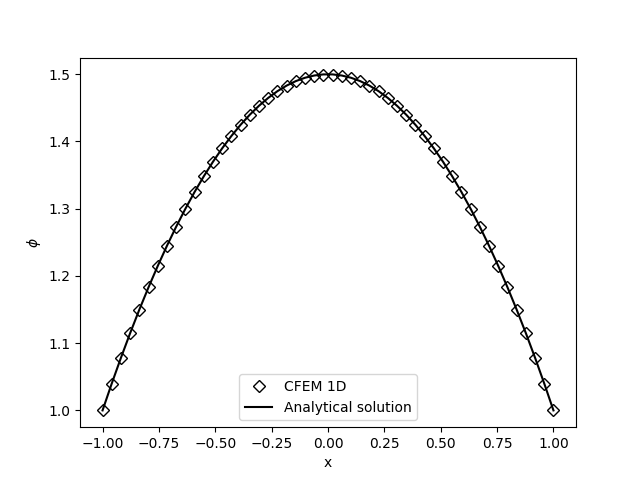
\includegraphics[width=0.8\linewidth]{Figures/Diffusion1a}
\caption{Comparison of CFEM solution to analytical solution.}
\label{fig:Diffusion1a}
\end{figure}

\subsubsection{Reflecting boundary condition}
Implementing a reflecting boundary condition cannot involve both boundaries being reflecting or else the system will be indeterminite. Therefore we will take the previous analytical solution and attempt to simulate the right half.

\begin{equation*}
\begin{aligned}
-\frac{\partial}{\partial x} \frac{\partial \phi}{\partial x} = 1 \quad \quad \forall x \in [-1,1] \\
\frac{\partial \phi}{\partial x}\biggr |_{x=0} = 0 \quad \quad \text{on } \partial \bOmega \\
\phi(1) = 1 \quad \quad \text{on } \partial \bOmega
\end{aligned}
\end{equation*}

The analytical solution is still

\begin{equation*}
\begin{aligned}
\phi(x) = -\frac{1}{2}x^2 + \frac{3}{2} \\
\end{aligned}
\end{equation*}

The results are shown in Figure \ref{fig:Diffusion1b} below.

\begin{figure}[H]
\centering
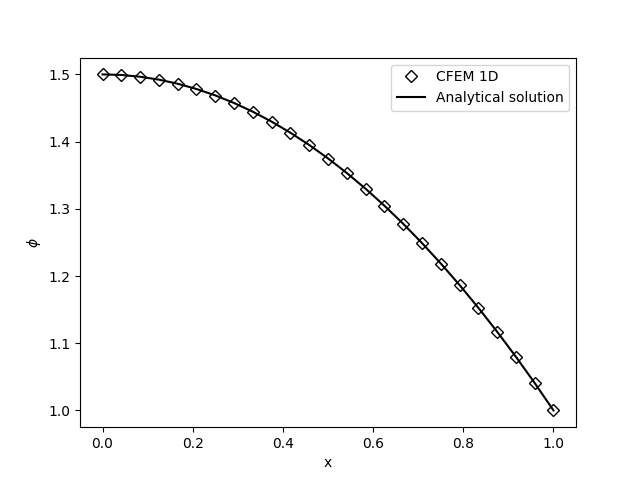
\includegraphics[width=0.8\linewidth]{Figures/Diffusion1b}
\caption{Comparison of CFEM solution to analytical solution using a reflecting boundary.}
\label{fig:Diffusion1b}
\end{figure}

\subsubsection{Vacuum boundary conditions}
For vacuum boundary conditions we deal with the following

\begin{equation*}
\begin{aligned}
-\frac{\partial}{\partial x} \frac{\partial \phi}{\partial x} = 1 \quad \quad \forall x \in [-1,1] \\
\frac{1}{4}\phi + \frac{1}{2}D \hat{n} \cdot \frac{\partial \phi}{\partial x} = 0 \quad \quad \text{on } \partial \bOmega \\
\end{aligned}
\end{equation*}

The results are shown in Figure \ref{fig:Diffusion1c}.

\begin{figure}[H]
\centering
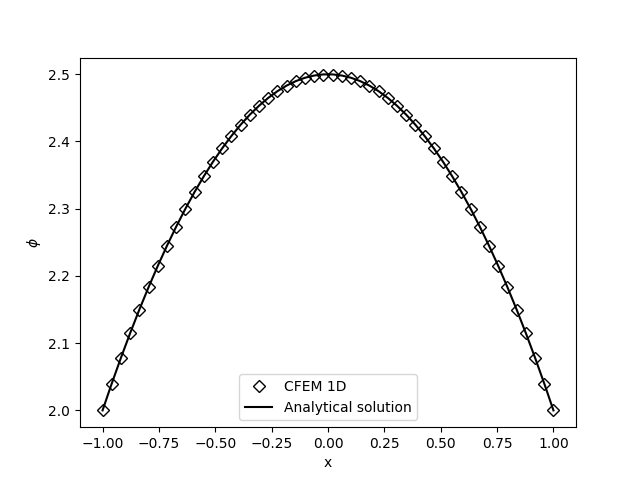
\includegraphics[width=0.8\linewidth]{Figures/Diffusion1c}
\caption{Comparison of CFEM solution to analytical solution using vacuum boundary conditions.}
\label{fig:Diffusion1c}
\end{figure}

\newpage
\section{Modified Interior Penalty}
Instead of a Continuous Finite Element Method (CFEM) discretization, 
where the solution is defined on nodes, the Discontinuous Finite Element
Method (DFEM) stores values per cell. More specifically, using Piecewise
Linear (PWL) basis functions and trial functions, defines the solution per cell 
node. The complication with using this formulation is then that the 
connectivity between cells is not as easy to determine as it was for 
CFEM discretization.

The weak form of the diffusion equation is extended as can be observed 
in the paper by Ragusa, repeated here, the interior penalty method matrix takes on the form
\begin{equation*}
\begin{aligned}
a(\delta \phi,b_i) &= 
(\sigma_a \delta \phi, b_i)_{\mathcal{D}} + 
(D\nabla \delta \phi,\nabla b_i)_{\mathcal{D}} \\
&+ 
(\kappa^{MIP} \llbracket \delta \phi \rrbracket,\llbracket b_i \rrbracket)_f +
(\llbracket \delta \phi \rrbracket,\ldblbrace D \partial_n b_i \rdblbrace)_f +
(\ldblbrace D \partial_n \delta \phi \rdblbrace,\llbracket b_i \rrbracket)_f \\
&+
(\kappa^{M I P} \delta \phi, b_{i})_{\partial \mathcal{D}} -
\frac{1}{2}(\delta \phi, \mathrm{D} \partial_{n} b_{i})_{\partial \mathcal{D}}-
\frac{1}{2}(\mathrm{D} \partial_{n} \delta \phi, b_{i})_{\partial \mathcal{D}}
\end{aligned}
\end{equation*}
\newline
where the jump and average operators are defined across an interface as
\begin{equation*}
\begin{aligned}
\llbracket u \rrbracket &= u^+ - u^- \\
\ldblbrace u \rdblbrace &= \frac{1}{2}(u^+ + u^-)
\end{aligned}
\end{equation*}
\newline 
The definition of $\kappa^{MIP}$ is discussed in a later section.
The $\pm$ is associated with the sense the given cell has with the given 
face, i.e. if the face has the righthand-rule convention and consistency 
with the normal then the cell that has a negative sense to it is the 
cell to which this convention is consistent. For our purposes we will 
denote $cell^-$ as the ``current"-cell and $cell^+$ as the ``adjacent"-cell.
\newline 
\newline
Other notations used here are the volume integrals, $(F)_{\mathcal{D}}$, 
integration over interior faces $(F)_f$, and integration over face 
exterior faces $(F)_{\partial \mathcal{D}}$ on the boundary of the domain.
\newline 
\newline
To assemble the matrix entries using this formulation we can replace $\delta \phi$ with $b_j$ to find

\begin{equation*}
\begin{aligned}
a(b_j,b_i) &= 
(\sigma_a b_j, b_i)_{\mathcal{D}} + 
(D\nabla b_j,\nabla b_i)_{\mathcal{D}} \\
&+ 
(\kappa^{MIP} \llbracket b_j \rrbracket,\llbracket b_i \rrbracket)_f +
(\llbracket b_j \rrbracket,\ldblbrace D \partial_n b_i \rdblbrace)_f +
(\ldblbrace D \partial_n b_j \rdblbrace,\llbracket b_i \rrbracket)_f \\
&+
(\kappa^{M I P} b_j, b_{i})_{\partial \mathcal{D}} -
\frac{1}{2}(b_j, \mathrm{D} \partial_{n} b_{i})_{\partial \mathcal{D}}-
\frac{1}{2}(\mathrm{D} \partial_{n} b_j, b_{i})_{\partial \mathcal{D}}
\end{aligned}
\end{equation*}
\newline 
Let us now develop these terms part-by-part. Imagine 3 terms, corresponding to the terms that have
either $\llbracket \rrbracket$ or $\ldblbrace \rdblbrace$, which will be termed part A, B and C.

\newpage
\subsection{Part A}
Part A then becomes
\begin{equation*}
\begin{aligned}
(\kappa^{MIP} \llbracket b_j \rrbracket,\llbracket b_i \rrbracket)_f = 
\int_f \kappa^{MIP} \llbracket b_j \rrbracket,\llbracket b_i \rrbracket .dA
\end{aligned}
\end{equation*}
Now, for simplicity let us replace $\kappa^{MIP}$ with $K$ and only focus on the terms inside
the integral, part A now becomes

\begin{equation}
\begin{aligned}
&\quad \kappa^{MIP} \llbracket b_j \rrbracket,\llbracket b_i \rrbracket \\ 
&= K (b_j^+ - b_j^-)(b_i^+ - b_i^-) \\
&= K (b_i^+ - b_i^-) b_j^+ - K (b_i^+ - b_i^-) b_j^-  \\
&= K (b_i^+ - b_i^-) b_j^+ \quad + \Aboxed{K (b_i^- - b_i^+) b_j^-} .
\end{aligned}
\end{equation}
\newline 
The assembly of the interface terms into the matrix is a very complicated
 process. Each interface has to update each cell belonging to the 
 interface. This is further complicated by the nominal way in which the
 matrix is normally assembled, i.e. cell-by-cell. Fortunately, some 
 symmetry exists within the different parts as can be seen in part A above.
 The boxed portion in the above code is symmetric to the unboxed portion
 with respect to the cell with a negative sense to the face. In other words
 if we loop cell by cell and only execute the boxed portion, this will be
 equivalent to looping over the interfaces and updating both sides.

Given we computed $K$ we can now calculate the following on the interface
based on our current cell location ($cell^-$)

\begin{equation}
\begin{aligned}
& \quad (\kappa^{MIP} \llbracket b_j \rrbracket,\llbracket b_i \rrbracket)_{E_h^i} \\
&\text{for }i,j \text{ on current cell}\\
&\text{for }i^* \text{ on adjacent cell}\\
a_{i_rj_r} &= \biggr[ \kappa^{MIP} \int_{S_f} b_i.b_j.dA \biggr]_{cur-cell}\\
a_{i_r^*j_r} &= \biggr[ -\kappa^{MIP} \int_{S_f} b_{i^*}.b_j.dA \biggr]_{adj-cell},
\end{aligned}
\end{equation}

where $i_r$ and $j_r$ refers to the global matrix row and columns as 
mapped from the local matrices. The coding implementation for this is 
shown on the next page.
\newline
\newline
The implementation features a primary loop over trial space $i$ followed by a 
secondary loop over basis functions $j$. Since we are dealing only with the 
shape functions we loop over face dofs and map the face DOFs to cell DOFs using
the data \textbf{edge\_dof\_mappings}, developed during FE initialization. We
also use the ``interior penalty"-view of the cell to determine the matrix row
($ir$) corresponding to this cell's DOF-$i$. Since we are dealing with $b_i^*$ 
we also have to determine $i_r^*$, and hence we determine $i_{map}$ which is the
adjacent cell's DOF-$i$ index that corresponds to the current cell's DOF-$i$. 
The mapping of $i_{map}$ is then used with the adjacent cell's 
``interior penalty''-view to map to $i_r^*$. A similar procedure is applied to
the $b_j$ components but this time we are not dealing with indices on the adjacent
cell and therefore only $j_r$ is mapped. The values are inserted into global
matrix using PETSc's \textbf{MatSetValue} which need not refer to local values 
only.
\vspace{0.5cm}
\begin{lstlisting}[language=c++]
//========================= Assemble penalty terms
for (int fi=0; fi<num_face_dofs; fi++)
{
	int i  = fe_view->face_dof_mappings[f][fi];
	int ir = cell_ip_view->MapDof(i);

	//Mapping face index to adj-cell
	int imap = MapCellDof(adj_cell,poly_cell->edges[f][fi]);
	int irstar = adj_ip_view->MapDof(imap);

	for (int fj=0; fj<2; fj++)
	{
		int j  = fe_view->face_dof_mappings[f][fj];
		int jr = cell_ip_view->MapDof(j);

		double aij = kappa*fe_view->IntS_shapeI_shapeJ[f][i][j];

		MatSetValue(A,ir    ,jr, aij,ADD_VALUES);
		MatSetValue(A,irstar,jr,-aij,ADD_VALUES);
	}//for fj

}//for fi
\end{lstlisting}

\vspace{0.5cm}
\subsection{Part B}
Part B is 
\begin{equation*}
(\llbracket b_j \rrbracket,\ldblbrace D \partial_n b_i \rdblbrace)_f  =
\int_f \llbracket b_j \rrbracket,\ldblbrace D \partial_n b_i \rdblbrace .dA
\end{equation*}

Let us now expand the terms inside the integral

\begin{equation*}
\begin{aligned}
 &\llbracket b_j \rrbracket,\ldblbrace D \partial_n b_i \rdblbrace \\
 &= \frac{1}{2}\biggr(b_j^+ - b_j^-\biggr)\biggr(D^+\hat{n}\cdot\nabla b_i^+ + D^-\hat{n}\cdot\nabla b_i^-\biggr)\\
  &=\frac{1}{2}\biggr(D^+\hat{n}\cdot\nabla b_i^+ + D^-\hat{n}\cdot\nabla b_i^- \biggr)b_j^+
  - \frac{1}{2}\biggr(D^+\hat{n}\cdot\nabla b_i^+ + D^-\hat{n}\cdot\nabla b_i^- \biggr)b_j^-\\
 &=\frac{1}{2}\biggr(D^+\hat{n}\cdot\nabla b_i^+ + D^-\hat{n}\cdot\nabla b_i^-\biggr)b_j^+
 \Aboxed{
 - \frac{1}{2}\biggr(D^+\hat{n}\cdot\nabla b_i^+ + D^-\hat{n}\cdot\nabla b_i^-\biggr)b_j^-}
\end{aligned}
\end{equation*}
\newline
The blocked term in this equation is symmetric to the non-blocked terms with respect to the current cell and the adjacent cell. In other words, the normal ($\hat{n}$) in the blocked portion is with respect to the current cell ($cell^-$). When we flip the sign of all the $\pm$ denotations and set $\hat{n} = -\hat{n}$ then we obtain the non-blocked terms.
Some of the terms in the blocked portions can be combined with others so let us defer showing the code for that for now and proceed to part C.

\subsection{Part C}
Part C is
\begin{equation*}
(\ldblbrace D \partial_n b_j \rdblbrace,\llbracket b_i \rrbracket)_f  =
\int_f \ldblbrace D \partial_n b_j \rdblbrace,\llbracket b_i \rrbracket .dA
\end{equation*}

Let us now expand the terms inside the integral

\begin{equation*}
\begin{aligned}
 &\ldblbrace D \partial_n b_j \rdblbrace,\llbracket b_i \rrbracket \\
 &= \frac{1}{2}\biggr(b_i^+ - b_i^-\biggr)\biggr(D^+\hat{n}\cdot\nabla b_j^+ + D^-\hat{n}\cdot\nabla b_j^-\biggr)\\
 &= \frac{1}{2}\biggr(D^+\hat{n}\cdot\nabla b_j^+ + D^-\hat{n}\cdot\nabla b_j^-\biggr)b_i^+
- \frac{1}{2}\biggr(D^+\hat{n}\cdot\nabla b_j^+ + D^-\hat{n}\cdot\nabla b_j^-\biggr)b_i^-\\
 &= \frac{1}{2}\biggr(D^+\hat{n}\cdot\nabla b_j^+ + D^-\hat{n}\cdot\nabla b_j^-\biggr)b_i^+
 \Aboxed{
- \frac{1}{2}\biggr(D^+\hat{n}\cdot\nabla b_j^+ + D^-\hat{n}\cdot\nabla b_j^-\biggr)b_i^-}
\end{aligned}
\end{equation*}
\newline
Again the same symmetry applies as with part B (i.e. flipping the denotations and the signs on the normals).

\subsection{Assembling B and C}
We first look at the blocked parts of B and C together

\begin{equation*}
\begin{aligned}
 &\Aboxed{
  - \frac{1}{2}\biggr(D^+\hat{n}\cdot\nabla b_i^+ + D^-\hat{n}\cdot\nabla b_i^-\biggr)b_j^-} \quad
 \Aboxed{
- \frac{1}{2}\biggr(D^+\hat{n}\cdot\nabla b_j^+ + D^-\hat{n}\cdot\nabla b_j^-\biggr)b_i^-}\\
\end{aligned}
\end{equation*}

\begin{equation*}
\begin{aligned}
&=
- \frac{1}{2} b_j^- D^+\hat{n}\cdot\nabla b_i^+ \quad
- \frac{1}{2} b_j^- D^-\hat{n}\cdot\nabla b_i^- \quad
- \frac{1}{2} b_i^- D^+\hat{n}\cdot\nabla b_j^+ \quad
- \frac{1}{2} b_i^- D^-\hat{n}\cdot\nabla b_j^- 
\end{aligned}
\end{equation*}
\newline
We now reshuffle the terms here after first noting that the second and last terms are the transpose of each other as well as the first and third.

\begin{equation*}
\begin{aligned}
&=
- \frac{1}{2} b_j^- D^-\hat{n}\cdot\nabla b_i^- \quad
- \frac{1}{2} b_i^- D^-\hat{n}\cdot\nabla b_j^- \quad
- \frac{1}{2} b_j^- D^+\hat{n}\cdot\nabla b_i^+ \quad
- \frac{1}{2} b_i^- D^+\hat{n}\cdot\nabla b_j^+ 
\end{aligned}
\end{equation*}
\newline
We now reintroduce the surface integrals

\begin{equation*}
\begin{aligned}
&\int_f \biggr[
- \frac{1}{2} b_j^- D^-\hat{n}\cdot\nabla b_i^- \quad
- \frac{1}{2} b_i^- D^-\hat{n}\cdot\nabla b_j^- \quad
- \frac{1}{2} b_j^- D^+\hat{n}\cdot\nabla b_i^+ \quad
- \frac{1}{2} b_i^- D^+\hat{n}\cdot\nabla b_j^+ 
\biggr].dA \\
&=- \frac{1}{2} D^-\hat{n} \cdot \int_f \biggr(
b_j^- \cdot\nabla b_i^- +
b_i^- \cdot\nabla b_j^-
\biggr).dA \quad
- \frac{1}{2} D^+\hat{n}\cdot  \int_f \biggr(
b_j^- \cdot\nabla b_i^+
\biggr).dA \quad
- \frac{1}{2} D^+\hat{n}\cdot  \int_f \biggr(
b_i^- \cdot\nabla b_j^+
\biggr).dA
\end{aligned}
\end{equation*}
\newline
Theoretically the two right hand integrals could have been lumped in a similar fashion to the left-most integral, however, this segregation proved useful for efficiency in the looping structure with minimal mapping. We therefore have the following three equations to implement

\begin{equation}
a_{i_r,j_r} = 
- \frac{1}{2} D^-\hat{n} \cdot \int_f \biggr(
b_j^- \cdot\nabla b_i^- +
b_i^- \cdot\nabla b_j^-
\biggr).dA
\end{equation}

\begin{equation}
a_{i_r^*,j_r} = 
- \frac{1}{2} D^+\hat{n}\cdot  \int_f \biggr(
b_j^- \cdot\nabla b_i^+
\biggr).dA
\end{equation}

\begin{equation}
a_{i_r,j_r^*} = 
- \frac{1}{2} D^+\hat{n}\cdot  \int_f \biggr(
b_i^- \cdot\nabla b_j^+
\biggr).dA
\end{equation}
\newline
The coding implementation is shown below:

\vspace{0.5cm}
\begin{lstlisting}[language=c++]
// -Di^- bj^- and
// -Dj^- bi^-
for (int i=0; i<fe_view->dofs; i++)
{
  int ir = cell_ip_view->MapDof(i);

  for (int j=0; j<fe_view->dofs; j++)
  {
    int jr = cell_ip_view->MapDof(j);

    double gij =
      n.Dot(fe_view->IntS_shapeI_gradshapeJ[f][i][j] +
            fe_view->IntS_shapeI_gradshapeJ[f][j][i]);
    double aij = -0.5*diffCoeff*gij;

    MatSetValue(A,ir,jr,aij,ADD_VALUES);
  }//for j
}//for i
\end{lstlisting}

\vspace{0.25cm}
\begin{lstlisting}[language=c++]
// - Di^+ bj^-
for (int imap=0; imap<adj_fe_view->dofs; imap++)
{
  int irmap = adj_ip_view->MapDof(imap);

  for (int fj=0; fj<num_face_dofs; fj++)
  {
    int jmap  = MapCellDof(adj_cell,poly_cell->edges[f][fj]);
    int j     = MapCellDof(poly_cell,poly_cell->edges[f][fj]);
    int jr    = cell_ip_view->MapDof(j);

    double gij =
      n.Dot(adj_fe_view->IntS_shapeI_gradshapeJ[fmap][jmap][imap]);
    double aij = -0.5*diffCoeff*gij;

    MatSetValue(A,irmap,jr,aij,ADD_VALUES);
  }//for j
}//for i
\end{lstlisting}

\vspace{0.25cm}
\begin{lstlisting}[language=c++]
// - Dj^+ bi^-
for (int jmap=0; jmap<adj_fe_view->dofs; jmap++)
{
  int jrmap = adj_ip_view->MapDof(jmap);

  for (int fi=0; fi<num_face_dofs; fi++)
  {
    int imap  = MapCellDof(adj_cell,poly_cell->edges[f][fi]);
    int i     = MapCellDof(poly_cell,poly_cell->edges[f][fi]);
    int ir    = cell_ip_view->MapDof(i);

    double gij =
      n.Dot(adj_fe_view->IntS_shapeI_gradshapeJ[fmap][imap][jmap]);
    double aij = -0.5*diffCoeff*gij;

    MatSetValue(A,ir,jrmap,aij,ADD_VALUES);
  }//for j
}//for i
\end{lstlisting}

\newpage
\chead{References}
\begin{thebibliography}{1}
    
    \bibitem{blender} {\em Blender - a 3D modelling and rendering package}, Blender Online Community, Blender Foundation, Blender Institute, Amsterdam, 2018
    
    \bibitem{delaunay} Cheng et al, {\em Delaunay Mesh Generation}, Chapman \& Hall/CRC Computer \& Information Science Series, 2013
    
    
\end{thebibliography}





\end{document}